%% LyX 2.0.6 created this file.  For more info, see http://www.lyx.org/.
%% Do not edit unless you really know what you are doing.
\documentclass[english]{ctexbook}
\usepackage[top=3cm,bottom=3cm,left=1.5cm,right=2.2cm,headsep=10pt,a4paper]{geometry} % Page margins

\usepackage{fontspec}
\setcounter{secnumdepth}{3}
\setcounter{tocdepth}{3}
\usepackage{color}
\usepackage{babel}
\usepackage{wrapfig}
\usepackage{graphicx}
\usepackage[unicode=true,pdfusetitle, bookmarks=true,bookmarksnumbered=true,bookmarksopen=true,bookmarksopenlevel=1, breaklinks=false,pdfborder={0 0 1},backref=page,colorlinks=true]{hyperref}
%%\hypersetup{ unicode=false}
\usepackage{multirow}



%%%%%%%%%%%%%%%%%%%%%%%%%%%%%% LyX specific LaTeX commands.
%% Because html converters don't know tabularnewline
\providecommand{\tabularnewline}{\\}

\usepackage{fancyhdr}   
\pagestyle{fancy}

%双线页眉的设置                                                 
\makeatletter %双线页眉                                        
\def\headrule{{\if@fancyplain\let\headrulewidth\plainheadrulewidth\fi%
\hrule\@height 1.0pt \@width\headwidth\vskip1pt%上面线为1pt粗  
\hrule\@height 0.5pt\@width\headwidth  %下面0.5pt粗            
\vskip-2\headrulewidth\vskip-1pt}      %两条线的距离1pt        
\vspace{6mm}}     %双线与下面正文之间的垂直间距              
\makeatother  

\makeatother

\usepackage{xunicode}




\title{肿瘤基因组项目结题报告}
\author{基因组研究部 }



\begin{document}

\renewcommand{\contentsname}{目录}
\renewcommand{\figurename}{ 图}
\renewcommand{\tablename}{ 表}
\CTEXoptions[today=small]

\maketitle

\tableofcontents{}

\chapter{背景}
\section{项目背景}
样品信息:正常组织/肿瘤组织的子宫内膜癌样本
\section{研究思路}
样本选择:
测序策略: Illumina HiSeq2000 PE100测序;

信息分析:SNP检测、InDel检测、SV检测、CNV检测、癌基因检测、临床分析(与变异相关的药效信息);

扩大样本验证:对扩大样本验证的建议

功能实验:对后续功能实验的建议


\chapter{研究方法}


\section{实验流程}


\subsection{样品提取}

冰冻样本/石蜡样本


\subsection{建库及测序}

样品接受与检验:样品到达后,首先进行Nanodrop和Qubit检测。A260/A280在1.8\textasciitilde{}2.0之间,含量在3ug以上的DNA样品才能用来进行建库。

基因组DNA片段的获取:检验合格的DNA样品通过Covaris破碎机随机打断成长度为500bp的片段。

文库构建:采用TruSeq Library Construction Kit 进行建库,严格使用说明书推荐的试剂和耗材。DNA片段经末端修复、加ployA尾、加测序接头、纯化、PCR扩增等步骤完成整个文库制备。

IlluminaHiSeq2000测序: 构建好的文库通过IlluminaHiSeq2000进行测序


\section{数据分析流程}


\subsection{数据质控}

Hiseq2000测序得到的原始图像数据经base calling 转化为序列数据,我们称之为raw data 或 raw reads,结果以fastq文件格式存储(文件名:{*}.fq)。Raw
data中会包含接头信息,低质量碱基,未测出的碱基(以N表示),这些信息会对后续的信息分析造成很大的干扰,分析前需要将这些干扰信息去除掉,最终得到的数据即为有效数据,我们称之为clean
data 或clean reads。原始数据过滤方法如下: (1). 过滤掉含有接头序列的 reads; (2). 当单端测序read中含有的N的含量超过该条read长度比例的
10\% 时,需要去除此对paired reads; (3). 当单端测序 read 中含有的低质量(碱基质量值小于5)碱基数超过该条
read 长度比例的50\% 时,需要去除此对paired reads。 经过对测序数据的严格过滤,得到高质量的clean data。对产出数据进行统计,包括测序read数量,数据产量,测序错误率,Q20含量,Q30含量,GC含量等。


\subsection{比对}

有效测序数据通过BWA{[}1{]}软件比对到参考基因组(UCSC hg19){[}2{]} ,得到BAM{[}3{]}格式的最初的比对结果。
BAM文件再用Picard{[}4{]}和GATK{[}5{]} 进行去重复(duplicate removal)、局部重比对(local
realignment)、碱基质量值重校正(base quality recalibration)等处理,从而得到BAM格式的最终比对结果。
如果一个或一对read(s)在基因上可以有多个比对位置,BWA的处理策略是从中选择一个最好的,如果有两个或以上“最好”的比对位置,则从中随机选择一个。这种多重比对(multiple
hit)的处理对SNP、indel以及CNV等的检测有重要影响。通常检测SNP或INDEL的时候要使用高质量的比对(alignment),即比对质量值大于0或更高。


\subsection{变异检测}

Normal和Tumor的最终的BAM文件都用GATK的UnifiedGenotyper模块进行SNP/INDEL的检测。CNVnator{[}6{]}利用深度(depth)信号来检测拷贝数增加或减少;BreakDancer{[}7{]}用PE关系(PE
mapping)的策略检测插入、删除、倒位和转座等;pindel{[}8{]}用切分(split read)的策略检测插入、删除、串联重复和倒位等。

直接比较Normal和Tumor,可以检测体细胞突变。从VarScan检测的结果过率掉群体中的多态性位点(来自dbSNP)得到最后的点突变;用GATK的SomaticIndelDetector模块检测小的插入缺失,也过滤掉群体中的多态性位点;Tumor中的拷贝数改变用FREEC检测;另外用breakdancer和pindel检测其它体细胞结构突变(\ref{info_pipeline})。

\begin{figure}[htbp]
\label{info_pipeline}
\centering
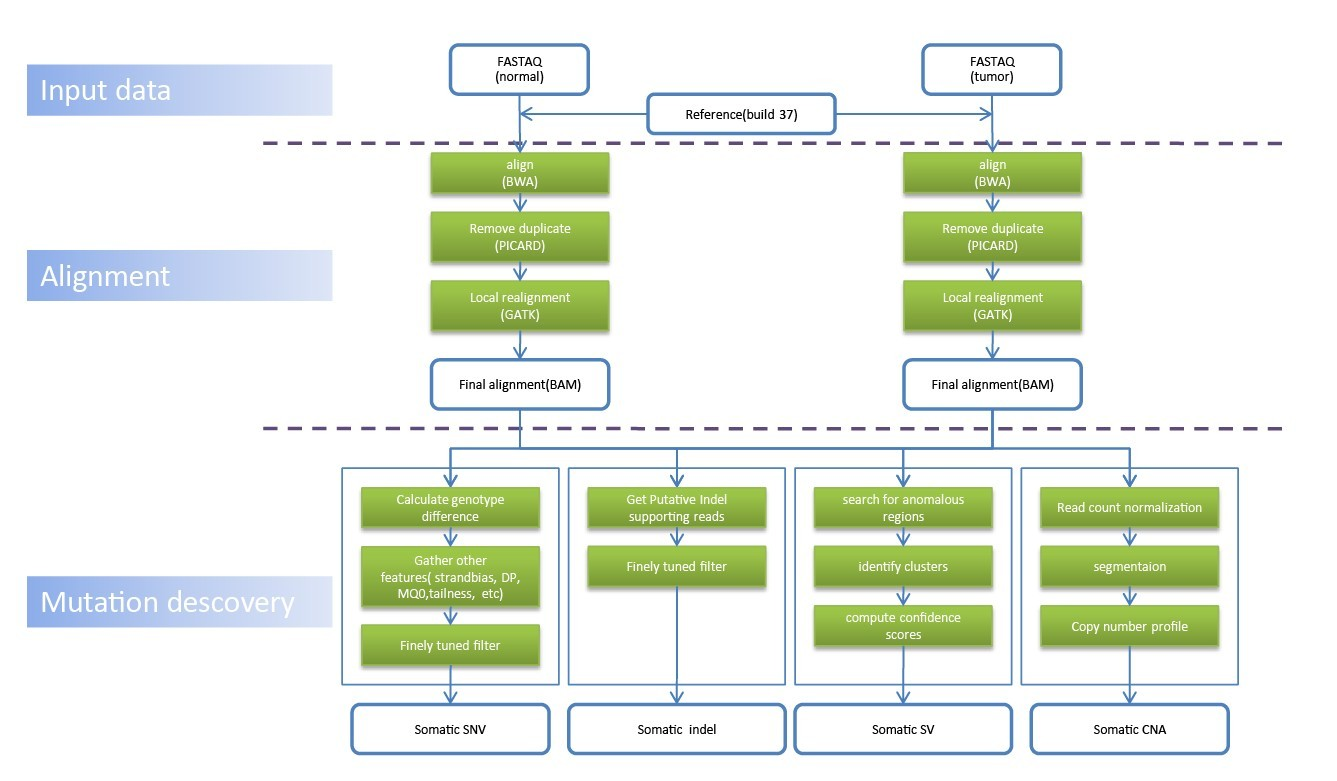
\includegraphics[width=0.8\textwidth]{001}
\caption{体细胞突变分析流程}
\end{figure}


\subsection{功能注释}

检测出的变异用UCSC的注释数据库,dbSNP,GWAS关联位点目录,药物敏感性数据集,疾病和癌症基因集,COSMIC,KEGG,GO等数据库进行注释。 


\chapter{结果}


\section{测序结果}

统计测序碱基A、T、C、G、N的含量,碱基分布均匀(图)。N含量小于该条read长度比例的10\%。 测序错误率与碱基质量有关,根据测序技术的特点,测序片段末端的错误率会偏高,并且大片段文库测序的错误率比小片段文库测序的错误率高。测序量,Q20,Q30,GC含量等的统计见表\ref{data_production}。

将clean data与NCBI的NT数据库进行比对,未发现其他来源的DNA污染。 


\begin{table}[htbp]
\label{data_production}
\centering
\caption{data production}
{ \zihao{6}
%%TABLE:data_production
}
\end{table}

通常,人类样本的测序read能达到95\%以上的比对率;10X以上read覆盖的位点检测出的SNP比较可信。统计样本的比对率,覆盖率,平均覆盖深度等如表\ref{mapping_stat}和图\ref{depth_dist}。
根据X、Y染色体的覆盖深度,可以看出所测样本的性别(图\ref{byChr_depth_dist})。

\begin{table}[htbp]
\label{mapping_stat}
\centering
\caption{比对率和覆盖度统计}
{ \zihao{6}
%%TABLE:mapping_stat
}
\end{table}

\begin{figure}[htbp]
\label{depth_dist}
\centering
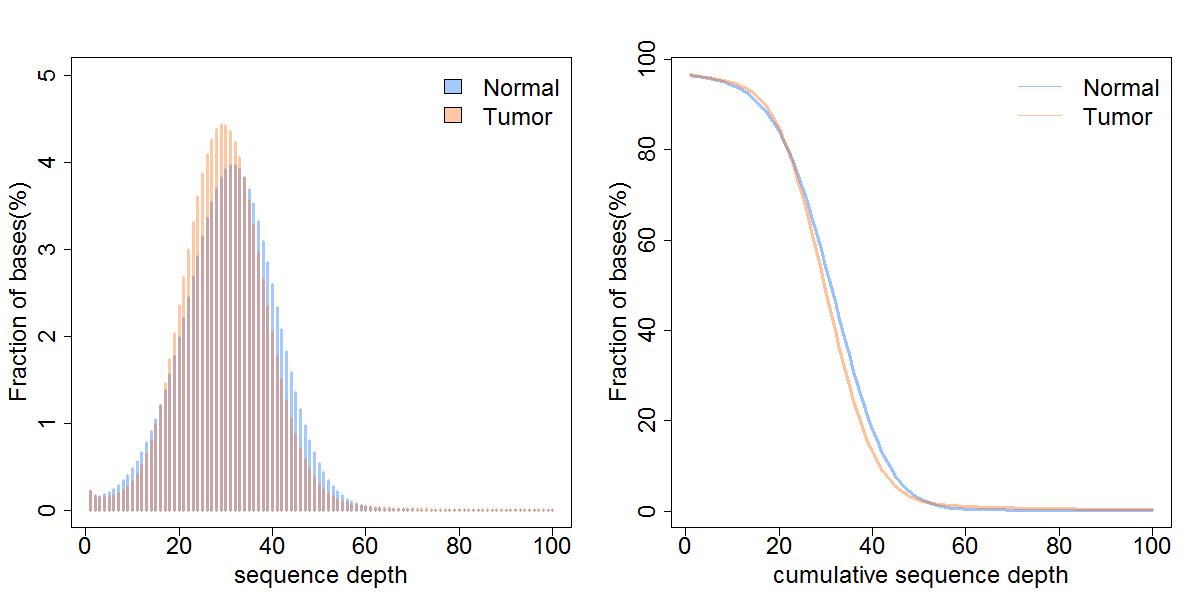
\includegraphics[width=0.8\textwidth]{depth}
\caption{测序深度}
\end{figure}

\begin{figure}[htbp]
\label{byChr_depth_dist}
\centering
\includegraphics[width=0.8\textwidth]{covByChr}
\caption{每个染色体的深度分布}
\end{figure}


\section{基因组上的变异结果}
\subsection{变异}

%%\paragraph{概述}
通常,个人全基因组内会有约3.6M个SNP[9],绝大数(大于95\%)的高频(群体中等位基因频率大于5\%)的SNP在dbSNP中有记录。转换/颠换的比值(Ts:Tv)可以反应SNP数据集的准确性,全基因内的比值约在2.2左右,编码区内的比值约在3.2左右。
样本中的SNP检测结果如表\ref{snp_stat}。


\begin{table}[htbp]
\label{snp_stat}
\centering
\caption{SNP检测结果}
{ \zihao{6}
%%TABLE:snp_stat

}
\end{table}

通常,个人全基因组内会有约350K的INDEL[9](INsertion and DELetion,小于50bp的插入缺失),其中约60\%的INDEL会在dbSNP里有记录。
样本中INDEL的检测结果如表\ref{indel_stat}。

\begin{table}[htbp]
\label{indel_stat}
\centering
\caption{indel检测结果}
{ \zihao{6}
%%TABLE:indel_stat

}
\end{table}

移码变异,其插入或缺失的碱基串的长度非3的整数倍,因此可能导致整个读框的改变;与非移码变异比较,受到的限制更大。这可以在INDEL的长度分布中反应出来(图 6)。

\subsection{变异的功能}

剪接位点上的变异,或无义突变会导致不正确的蛋白质翻译。其他非同义改变也有可能改变蛋白的功能。用SIFT[11]、PolyPhen2[12]对非同义改变的功能影响进行预测, 用GERP++预测保守位点的改变的影响,同时用千人基因组计划的群体频率信息细分SNP,结果汇总如图 9和表 7。

GWAS目录中[13]的关联位点中,7,030个位点的检测出的基因型是高可信度的,其中1,778个是带有风险等位基因的。这些等位基因与352种表型相关联,131个与cancer或糖尿病相关联(表 7)。

与COSMIC[14]中的体细胞突变集比较,47个变异在COSMIC中有记录,其中7个为非同义突变,在群体中的等位基因频率小于0.01(表 9)。这些突变可能是会在肿瘤病人中复现的突变(recurrent mutation)。

搜索PharmGKB数据库[15],发现总共148个与药物敏感性有关的变异(表 10示例了其中一部分)。

\end{document}
